\documentclass[english,a4paper,11pt]{article}
\usepackage[margin=3cm]{geometry}
\usepackage[latin1]{inputenc}
\usepackage{babel}
\usepackage{bm}
\usepackage{amsmath,amsthm}
\usepackage{latexsym}
\usepackage{booktabs}
\usepackage[final]{graphicx}
\DeclareGraphicsExtensions{.jpg,.jpeg,.pdf,.png,.mps}
\usepackage{epsfig}
\usepackage[round]{natbib}
%\setcitestyle{aysep={}} 
\setcitestyle{numbers}
\setcitestyle{square}

%\usepackage[authoryear,comma,longnamesfirst,sectionbib]{natbib} 
\usepackage{rotating}
%\setlength{\topmargin}{-1cm}
\usepackage{color}
\usepackage{xcolor}
\usepackage{colortbl}
\usepackage[bitstream-charter]{mathdesign}
\usepackage[T1]{fontenc}
\usepackage{threeparttable}
\usepackage{lipsum}
\usepackage{url} 
\usepackage{hyperref}
\usepackage{lmodern}
\date{}
\hypersetup{hidelinks}

\addtolength{\textwidth}{1em}
\addtolength{\oddsidemargin}{-1em}

\linespread{1.2}

\usepackage[font=small,skip=5pt]{caption}

%% https://ies2025.sis-statistica.it/
\title{Transition Models for Precipitation Climatology Estimation}

\author{$\mathrm{Nikolaus \ Umlauf}^\mathrm{1},  
	\  \mathrm{Reto \ Stauffer}^\mathrm{1}$\\  
	$^\mathrm{1}$\small{\emph{Universtit\"at Innsbruck}}\\
}

\begin{document}

\maketitle

\begin{abstract}
Transition models are widely recognized for their flexibility in count data regression, where they
are known as continuation ratio models. They model transition probabilities--the conditional
probability of counts exceeding a threshold--using standard binary regression methods with an
augmented dataset.
This paper extends transition models to continuous data via a slicing technique that transforms
continuous observations into count-like data. This enables full probabilistic modeling,
including distributional, quantile, and modal regression, using simple binary regression methods.
The proposed method is highly adaptable, handling complex data structures like excess zeros
and non-standard distributions. We illustrate its usefulness with an application to precipitation
climatology estimation in Tyrol, Austria.
\noindent 
\hspace{1cm}\\
\emph{Keywords}:  transition models, distributional, quantile, and modal regression.
\end{abstract}

\section{Introduction}\label{sec:intro}

In many applications, the response variable is a count, often influenced by covariates.
Traditional models, such as Poisson and negative binomial regression, rely on fixed distributional
assumptions, which can lead to mis-specifications, particularly in the presence of overdispersion
or excess zeros. Various alternative distributions and modeling approaches have been proposed to
address these issues.
Transition models provide a powerful framework for count data estimation, offering flexibility
in capturing complex structures such as excess zeros and varying coefficients. Rather than assuming
a fixed distribution, they estimate the conditional probabilities of observing counts beyond a
given threshold, allowing the data to determine the underlying distribution. These probabilities
can be estimated via binary regression with augmented datasets, leveraging standard software
\cite{Berger:2021}. A key advantage of transition models is their ability to support both
parametric and nonparametric extensions, while simplifying estimation and enhancing interpretability.
This paper extends transition models to continuous data using a slicing technique that transforms
continuous observations into count-like data. This bridges traditional transition models with
advanced regression techniques, such as distributional, quantile and modal regression. The proposed
method effectively captures complex data structures and enables full probabilistic modeling using
standard binary regression tools. We illustrate its versatility with an application to
precipitation climatology estimation in Tyrol, Austria, highlighting its broader potential.

\section{Transition Models} \label{sec:tm}

Transition models provide a flexible framework for count data. We first introduce the classic
count model and then extend it to continuous responses.

\subsection{Classic Count Model} \label{sec:counts}

Transition models offer a flexible approach to count data by estimating conditional
transition probabilities rather than assuming a fixed distribution. This allows the data to
determine the response distribution.
Following \cite{Berger:2021}, let $y_i \in \{0, 1, 2, \dots\}$ be the count response for
observation $i$ with covariates $\mathbf{x}_i$. The transition probability is defined as  
\begin{equation} \label{eqn:tm}
P(y_i > r \mid y_i \geq r, \mathbf{x}_i) = F(\eta_{ir}(\boldsymbol{\alpha})), \quad r = 0, 1, \dots
\end{equation}
where $r$ denotes the count level, and $F(\cdot)$ is a cumulative distribution function (CDF),
such as the logistic or probit function. This probability describes a transition as
it models the likelihood of moving from count level $r$ to $r + 1$. The corresponding additive
predictor is given by 
$$
\eta_{ir}(\boldsymbol{\alpha}) = \theta_r + \sum_{j=1}^k f_j(\mathbf{x}_i, r; \boldsymbol{\beta}).
$$
The parameters $\boldsymbol{\alpha} = (\boldsymbol{\theta}^\top, \boldsymbol{\beta}^\top)$
include count-specific intercepts and smooth functions $f_j(\cdot)$, estimated via regression splines.
For i.i.d.\ observations, let $\pi_{ir}$ denote the probability that the count response equals $r$,
i.e., $P(y_i = r | \mathbf{x}_i)$. These probabilities are computed recursively as
$$
\pi_{ir} = (1 - F(\eta_{ir}(\boldsymbol{\alpha}))) \prod_{s=0}^{r-1} F(\eta_{is}(\boldsymbol{\alpha})).
$$
Parameter estimation considers the underlying Markov chain $Y_{i0}, Y_{i1}, \dots$,
where $Y_{ir} = \mathbb{1}(y_i = r)$. The log-likelihood simplifies to  
$$
\ell(\boldsymbol{\alpha}) = \sum_{i=1}^n \sum_{s=0}^{y_i} \Big[Y_{is} \log(1 - F(\eta_{ir})) + (1 - Y_{is}) \log(F(\eta_{ir}))\Big].
$$
This formulation arises from modeling the count response as a sequence of binary transitions,
where each step represents the probability of exceeding a given count level. It corresponds to a
binary model and can be estimated using generalized additive models (GAM, \cite{Wood17}).
Estimation is performed on an expanded dataset where binary responses
$(Y_{i0}, \dots, Y_{iy_i})^\top = (0, \dots, 0, 1)$ are created, along with a new
covariate $\boldsymbol{\Theta}_i = (0, 1, 2, \dots, y_i)^\top$ to capture
count-specific effects $f_j(\mathbf{x}_i, \boldsymbol{\Theta}_i)$, or simple count-specific
intercepts. All other covariates are duplicated accordingly.
While the dataset size increases, efficient GAM-based estimation methods for
large data \cite{Wood:2014, Wood:2017} mitigate computational costs. Alternatively, machine
learning approaches such as neural networks or random forests could be used.

\subsection{Continuous Responses} \label{sec:continuous}

To extend transition models to continuous responses $y_i \in \mathbb{R}$, we use a
discretization approach inspired by histogram binning. The response variable is divided
into $m - 1$ intervals using predefined bin boundaries $\zeta_1, \zeta_2, \dots, \zeta_m$,
where each interval $(\zeta_l, \zeta_{l+1}]$ corresponds to a discrete count $r$. Each observation
$y_i$ is assigned a pseudo count $\tilde{y}_i$ based on the interval it falls into, allowing the
transition model from Section~\ref{sec:counts} to be applied.

\subsubsection{Approximation of the CDF and Density}

The described discretization approach effectively provides a stepwise approximation of the
underlying smooth continuous distribution. For a continuous response variable $y_i$ with CDF $F(y)$,
the discretization process approximates the
probabilities of $y_i$ falling into each interval as
$P(\zeta_l < y_i \leq \zeta_{l+1}) = F(\zeta_{l+1}) - F(\zeta_l)$.
These probabilities are represented by the transformed counts $\tilde{y}_i$, allowing the
transition model to reconstruct the discrete probabilities as
$P(\tilde{y}_i = r) = P(\zeta_r < y_i \leq \zeta_{r+1})$.
The transition model estimates the probability of transitioning between counts
$$
P(\tilde{y}_i > r \mid \tilde{y}_i \geq r, \mathbf{x}_i) = F(\eta_{ir}(\boldsymbol{\alpha})),
$$
and recursively computes
$$
P(\tilde{y}_i = r, \mathbf{x}_i) = P(\tilde{y}_i = r \mid \tilde{y}_i \geq r, \mathbf{x}_i) \prod_{s=0}^{r-1} P(\tilde{y}_i > s \mid \tilde{y}_i \geq s, \mathbf{x}_i).
$$
For any value $y_i \in (\zeta_l, \zeta_{l+1}]$, the CDF can be approximated by
$$
\hat{F}(y_i) = \sum_{r=0}^{l-1} P(\tilde{y}_i = r) + \frac{y_i - \zeta_l}{\zeta_{l+1} - \zeta_l} P(\tilde{y}_i = l),
$$
where the first term sums probabilities for bins below $y_i$, and the second term performs
linear interpolation within the current bin. As the number of bins $m$ increases and bin
widths shrink, this stepwise approximation converges uniformly to the true CDF $F(y)$.
Similarly, the density function can be approximated as
$$
\hat{f}(y_i) = \frac{P(\tilde{y}_i = l)}{\zeta_{l+1} - \zeta_l}, \quad y_i \in (\zeta_l, \zeta_{l+1}].
$$

\subsubsection{Estimation of Key Distributional Properties}

Beyond estimating the CDF, the transition model allows for computing key
distributional characteristics. The mode is given by
$$
\hat{y}_i^* = \arg\max_r P(\tilde{y}_i = r \mid \mathbf{x}_i),
$$
with refinements possible through finer binning. The mean, variance, skewness, and kurtosis
can be estimated by weighting bin midpoints $\zeta_r$ with their corresponding probabilities:
$$
E[Y] = \sum_{r} \zeta_r P(\tilde{y} = r), \quad \text{Var}(Y) = E[Y^2] - (E[Y])^2,
$$
$$
\text{Skewness} = \frac{E[(Y - E[Y])^3]}{\text{Var}(Y)^{3/2}}, \quad \text{Kurtosis} = \frac{E[(Y - E[Y])^4]}{\text{Var}(Y)^2}.
$$

\subsubsection{Summary}

By transforming continuous data into a count-like representation, transition models enable
full probabilistic estimation, including distributional properties, in a computationally
efficient framework. This approach is particularly useful for applications requiring flexible
distributional modeling and probabilistic regression.

\section{Software} \label{sec:software}

The proposed method is implemented in the \textsf{R} package \textbf{transitreg} \cite{transitreg},
available on GitHub: \texttt{https://github.com/retostauffer/transitreg}. The development version
can be installed using
\begin{verbatim}
R> remotes::install_github("retostauffer/transitreg")
\end{verbatim}  
The main function for estimating transition models is \texttt{transitreg()}. A CRAN release is
planned for the near future.

\section{Application} \label{sec:application}

\begin{figure}[!ht]
\centering
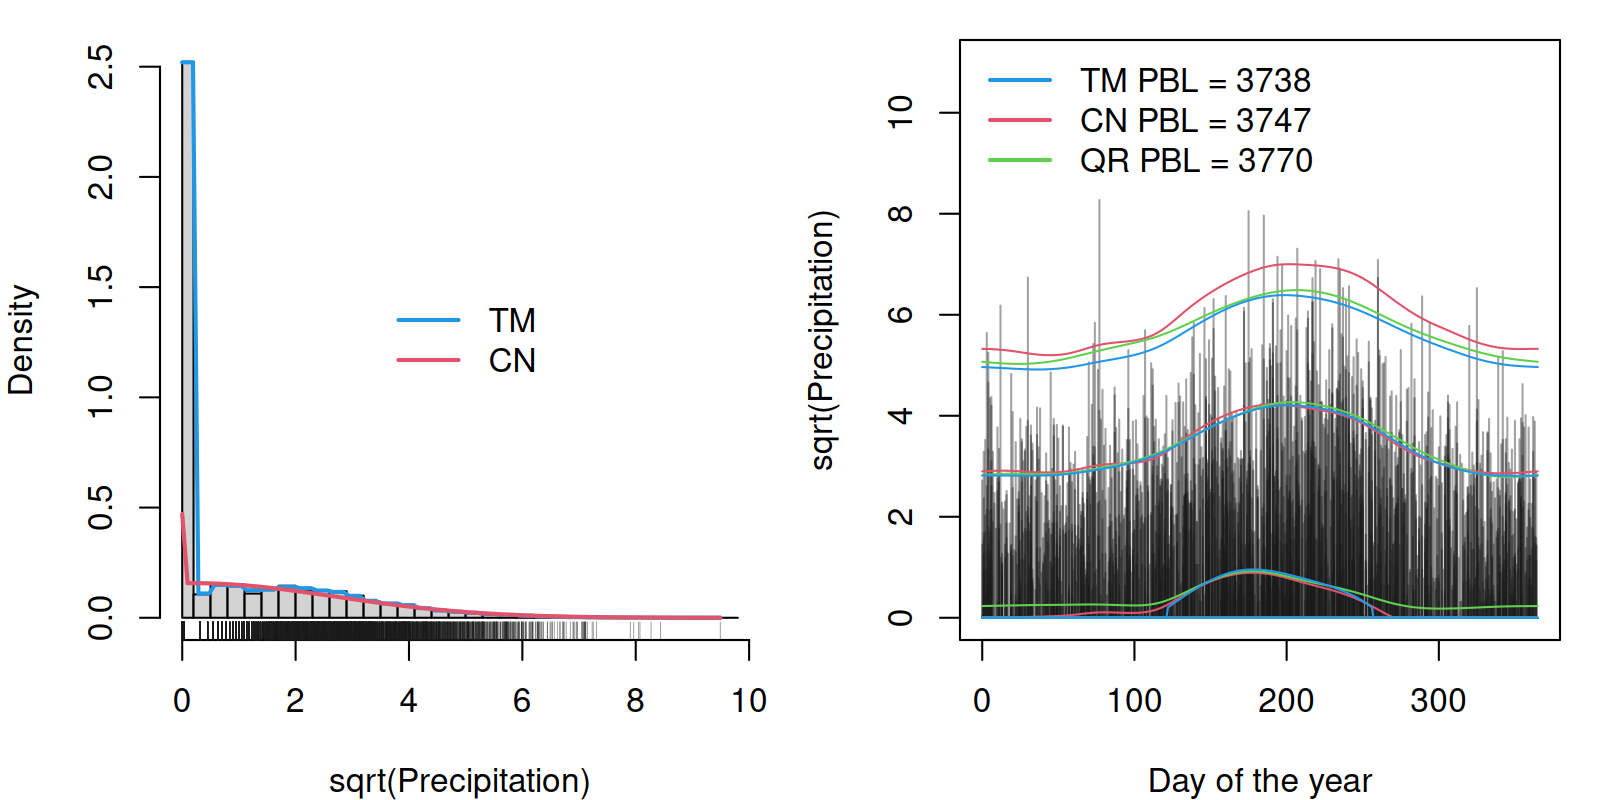
\includegraphics[width=0.9\textwidth]{ts_hist.png}
\caption{\label{fig:Kirchberg} Precipitation data for Kirchberg in Tirol, Austria.
  Left: Histogram of square root-transformed daily precipitation with fitted densities from a
  censored normal (CN, red) and transition model (TM, blue).
  Right: Seasonal variation in square root-transformed precipitation with empirical quantiles
  (1st, 10th, 50th, 90th, 99th percentiles) and out-of-sample quantile estimates for CN, TM, and
  quantile regression (QR), including their pinball loss (PBL) values.}
\end{figure}
\begin{figure}[!h]
\centering
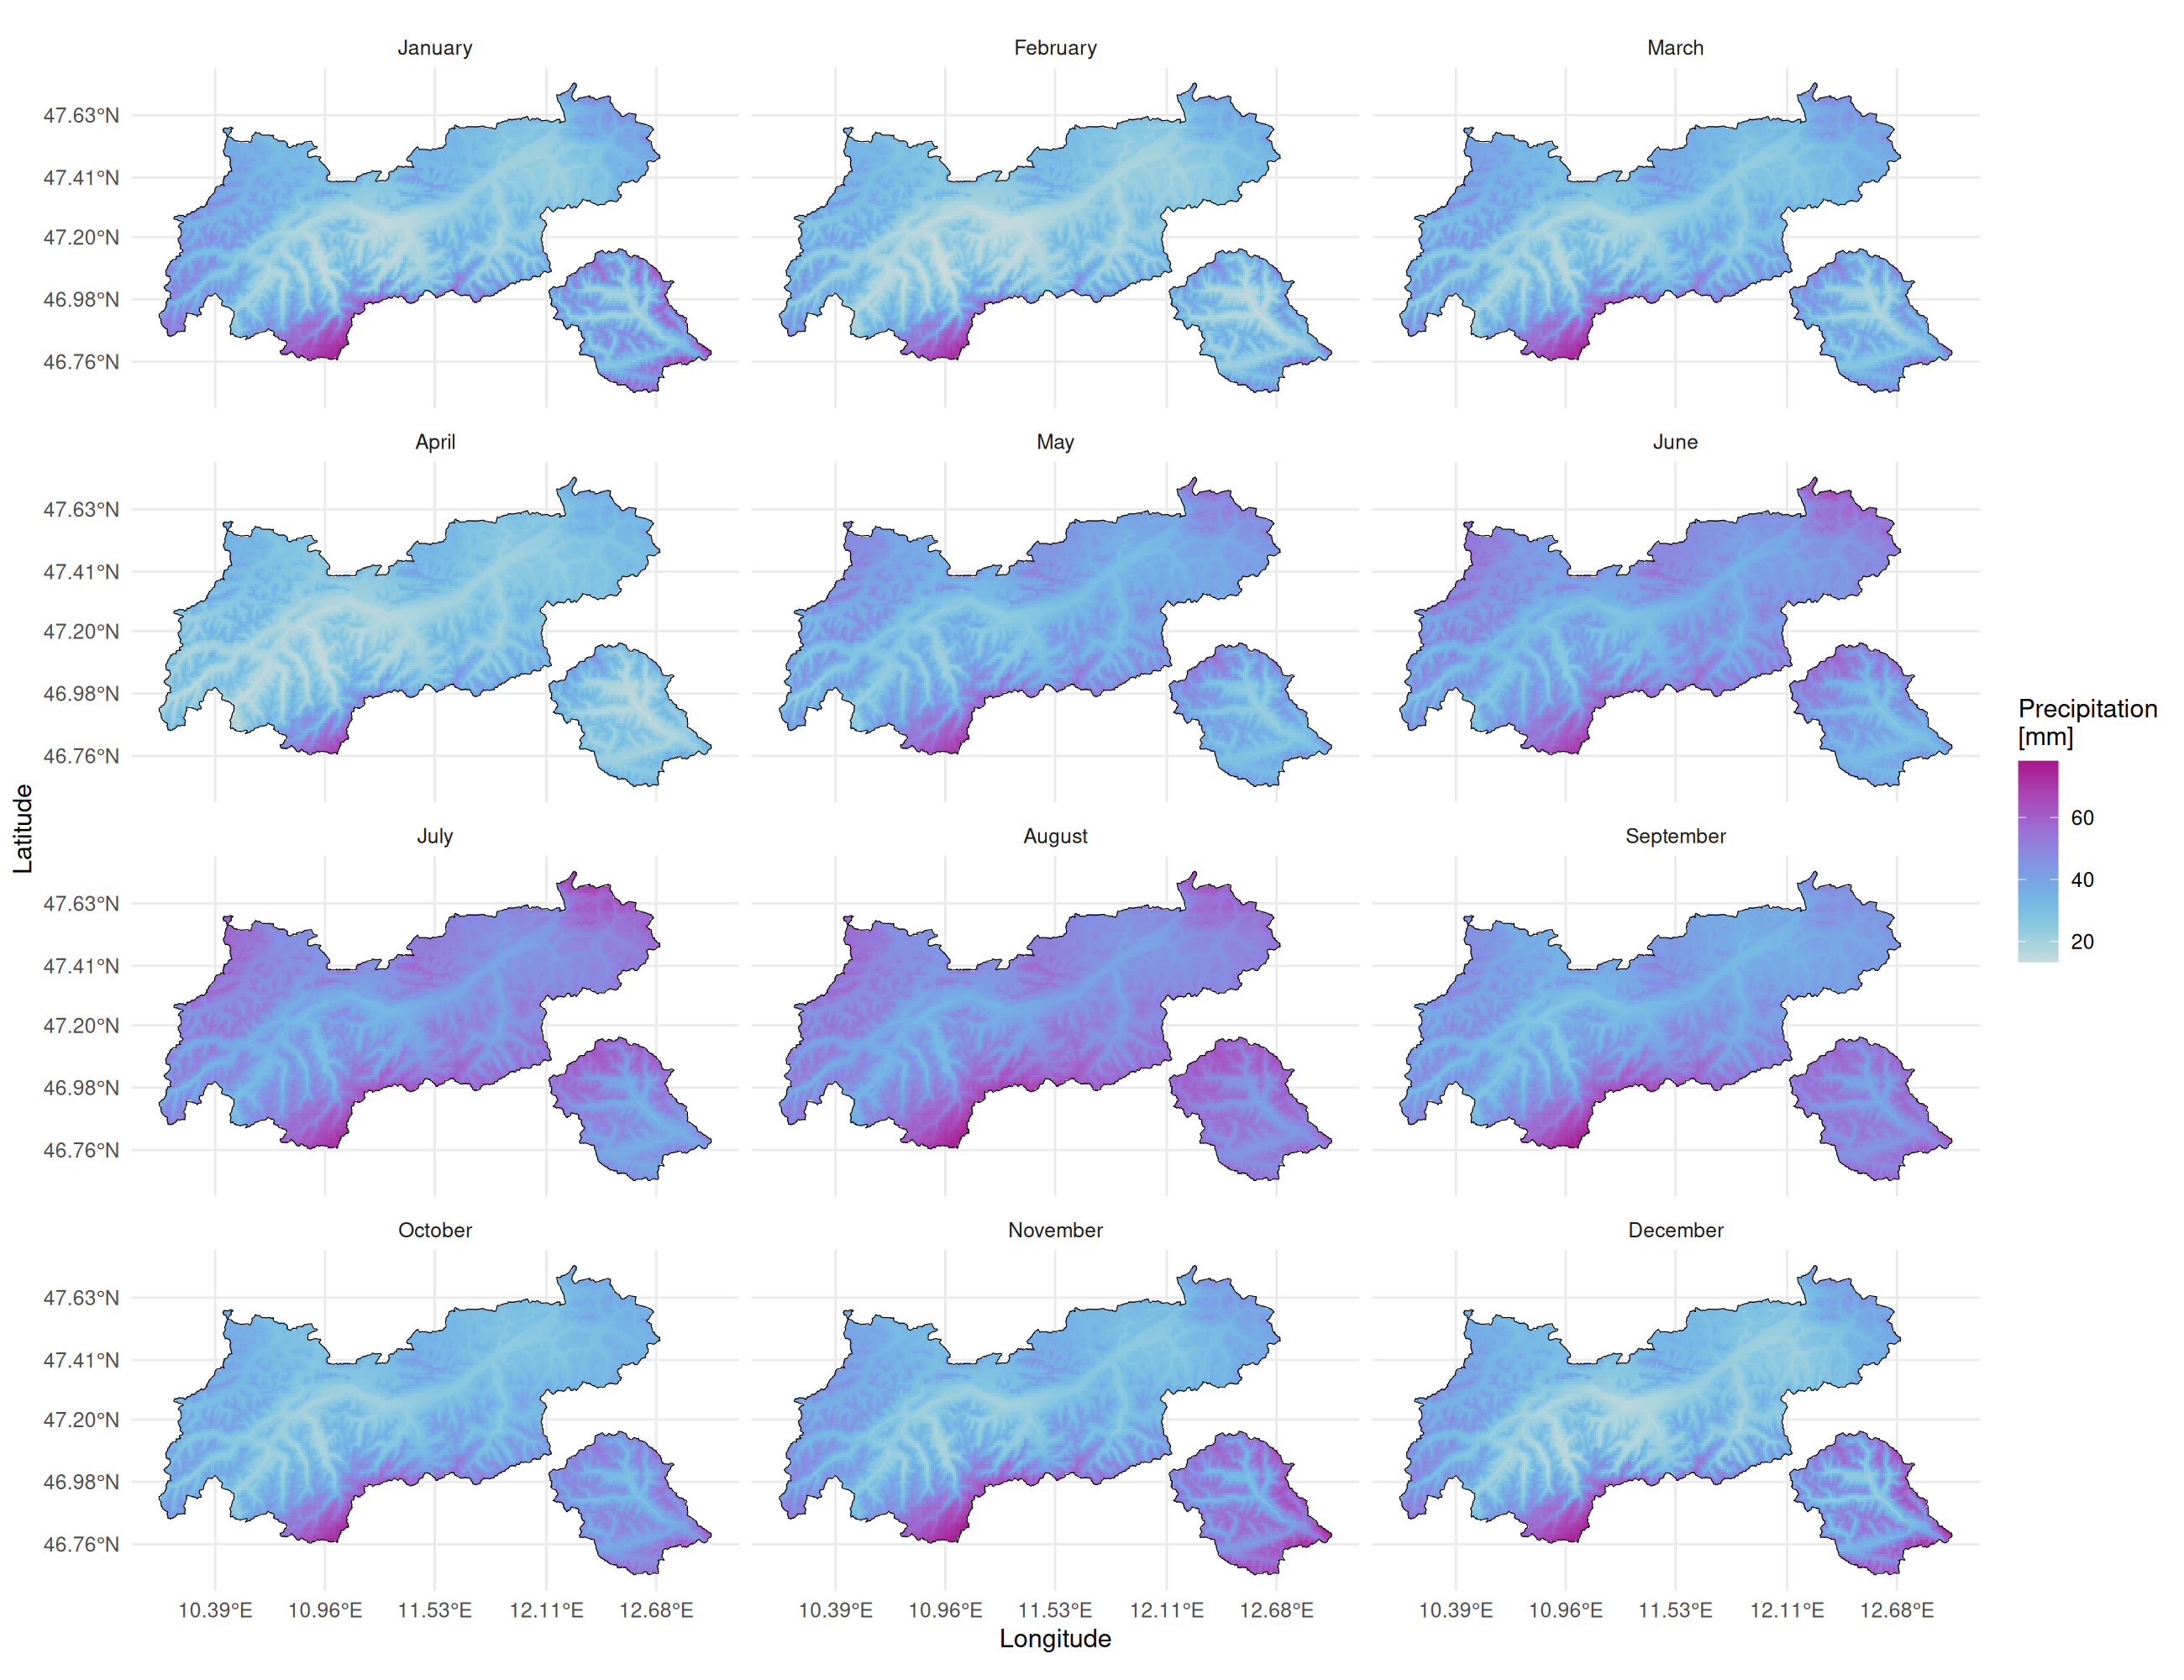
\includegraphics[width=1\textwidth]{predictions.png}
\caption{\label{fig:clim} Estimated climatology for the 99\% quantile precipitation using
  the TM model for selected days representing the 12 months of the year. The figure
  highlights spatial and seasonal variations in precipitation across Tyrol. Summer
  months exhibit the highest precipitation levels, whereas in winter, the southern
  regions experience the most precipitation.}
\end{figure}

In this application, we analyze 30 years of precipitation data (1992-2021)
from the Tyrolean Alps to estimate a 
climatology for precipitation. Figure~\ref{fig:Kirchberg} visualizes the raw data for the station 
Kirchberg in Tirol. The left panel presents a histogram of the square root-transformed precipitation 
values, overlaid with density estimates from a transition model (TM) and a parametric
censored normal (CN) model. Notably, the TM captures the inherent structure of the data more effectively, 
particularly the spike at zero precipitation. This demonstrates the flexibility of the TM approach, 
allowing it to directly model key features such as excess zeros.
The right panel displays out-of-sample precipitation data along with predicted quantiles. The 
corresponding pinball loss (PBL) values for the TM, CN, and quantile regression (QR) models are 
presented in the legend. Among these, the TM model provides the best prediction of the
out-of-sample distribution, as indicated by the lowest PBL. Notably, the 99\% quantile
predicted by the CN model is slightly higher than those of the TM and QR models, while
the 50\% quantile estimate from the QR model exceeds those of the TM and CN models.
Finally, to estimate a full climatology and validate the TM compared to the CN model, we split 
the data into training and testing sets by excluding 21 (20\%) of the total 105 meteorological 
stations from the training data. We computed the out-of-sample pinball loss (PBL) for the 0.01, 
0.1, 0.5, 0.9, and 0.99 quantiles. The TM achieved the lowest overall PBL of 221,442, compared 
to 221,570 for the CN. For the 99\% quantile, the TM's PBL was 1.21\% lower than the CN, 
demonstrating slightly better performance.
Although the transformed dataset used for the TM contained over 10 million observations, the 
estimation time was approximately 15 minutes, significantly faster than the 60 minutes required 
for the CN. The estimated climatology for the 99\% quantile using the TM is illustrated in 
Figure~\ref{fig:clim}, showing selected days of the year representing the 12 months. The figure 
highlights the TM's ability to capture space-time varying seasonal effects. Notably, the
highest precipitation amounts occur in the summer months, while in winter, the highest 
precipitation is concentrated in the southern parts of Tyrol.

\section{Conclusion} \label{sec:conclusion}

In this paper, we present an innovative application of transition models (TM) for estimating 
precipitation climatology, focusing on their flexibility and adaptability in handling complex 
data structures. Transition models, traditionally used for count data, are extended to 
continuous data using a slicing technique that transforms continuous observations into
count-like representations. This approach enables the estimation of full probabilistic models, 
including distributional, quantile and modal regression, using standard binary regression techniques.
Through an application to 30 years of precipitation data from Tyrol, Austria, we demonstrate
the robustness of the TM approach. The results show that the TM outperforms the censored normal 
(CN) model, achieving a lower pinball loss (PBL) across all quantiles.
For the critical 99\% quantile, the TM achieves a 1.21\% lower PBL compared to the CN,
while maintaining computational efficiency. The estimated climatology highlights seasonal 
precipitation variations, with summer months showing the highest precipitation levels
and winter precipitation concentrated in the southern regions of Tyrol.
This study underscores the potential of transition models for broader applications in 
probabilistic modeling, offering a computationally efficient and theoretically sound framework 
for analyzing complex data.

%\bibliographystyle{plainnat}
%\bibliographystyle{apalike}
\bibliographystyle{unsrt}
\bibliography{transitreg.bib}

%\listofchanges

\end{document}

